\documentclass[11pt]{article}
\usepackage[margin=1.03in]{geometry}
\usepackage{amsmath,amssymb,amsthm,booktabs,graphicx,microtype}
\usepackage{xcolor}
\usepackage[colorlinks=true,linkcolor=blue!50!black,citecolor=blue!50!black,urlcolor=blue!50!black]{hyperref}
\newtheorem{theorem}{Theorem}
\newtheorem{corollary}[theorem]{Corollary}
\newtheorem{proposition}[theorem]{Proposition}
\newcommand{\J}{J}
\newcommand{\E}{\mathcal E}
\newcommand{\HH}{\mathcal H}
\newcommand{\dd}{\mathrm d}
\title{How many states does a coarse junction need?\\Sharp bounds from two observation lags}
\author{Yunjie Guo \and Hanqing Yang\thanks{Corresponding author, \href{mailto:hanqing.yang189@gmail.com}{hanqing.yang189@gmail.com}. Affiliation for both authors: Independent Researcher, Suzhou, China.}}
\date{}
\begin{document}
\maketitle
\begin{abstract}
A reversible transport model may reproduce the traffic entering a coarse cell and still transmit mass between its neighbors too quickly. We determine the smallest two-step cross-port mass compatible with a given one-step traffic vector, cell mass and budget of hidden states inside the cell. For metric port costs the optimum is a partition of the ports followed by a scalar mass allocation. A reversible stochastic kernel attains it. For \(d\) equally loaded ports and \(k\le d\) hidden states the answer is \(\binom{d-k+1}{2}a^2/[M-(k-1)a]\), where \(a\) is one port's traffic and \(M\) the cell mass. The bound permits arbitrary hidden complexity outside the cell. We derive a distinct sharp curvature bound for reversible continuous-time networks and a finite-sample exclusion test using independent endpoint counts. A reflecting diffusion benchmark quantifies how observation lag, port geometry and sample size affect the number of states the data can certify.
\end{abstract}

\section{Coarse measurements and a local inverse problem}
Consider a finite-volume diffusion model that stores a single concentration in a junction and conserves the flux through each of its faces. An inflow through the west face immediately contributes to the concentration from which the other faces draw. A resolved cell can store that inflow near the west face for some time. How many internal concentrations must \emph{any} reversible Markov closure allocate to the junction to reproduce measured transfers? Repeating a fitted one-step coarse kernel and comparing the result with a two-step observation can reveal a discrepancy. Localizing the discrepancy to one cell is harder, since every neighboring cell may also have unresolved dynamics.

We use a finite state space, a stochastic kernel \(P\) and positive masses \(\pi_x\) satisfying \(\pi_x P_{xy}=\pi_y P_{yx}\). The mass scale is arbitrary. A continuous-time reversible process observed at a fixed interval has just such a kernel. The deterministic observation map records disjoint ports \(A_1,\ldots,A_d\) and a disjoint junction \(B\). Other states may be present. For any sets \(U,V\) define the observable
\[
 J_r(U,V)=\sum_{x\in U}\pi_x P^r(x,V),\qquad r=1,2.
\]
One can obtain it by initializing within \(U\) with probabilities proportional to \(\pi\), measuring the fraction in \(V\) at the target lag, and multiplying by \(\pi(U)\). Set \(M=\pi(B)\), \(a_i=J_1(B,A_i)\), and \(Y_W=\sum_{i<j}w_{ij}J_2(A_i,A_j)\). The symmetric costs \(w_{ij}\ge0\) have zero diagonal. We count each pair once. The state budget \(k\) counts all states in the preimage of \(B\), including the first coarse state. Neighboring aggregates may contain arbitrarily many states. Our question fixes only \(M,a\), the port masses, and this budget. Additional measured entries may exclude models that pass this test.

In aggregated-process theory, counting exponential components in a dwell-time distribution gives a lower bound on the number of states in the observed aggregate \cite{fredkin}. Projected Markov models separate a Markov process in full state space from its observed kinetics and motivate fitting hidden states \cite{noe}. Positive and linear realization theory uses past--future factorizations \cite{vidyasagar}, while nonnegative low-rank aggregation can estimate the number of metastates from a full transition matrix \cite{duan}. Here a local budget must constrain a weighted scalar at lag two even when every exterior aggregate is free to change. The midpoint factorization below is classical. Our result solves its extremal problem with prescribed \emph{local} one-lag marginals and gives a matching Markov construction. The partition objective also relates to weighted Gini impurity \cite{cicalese}. The unused one-step probability in each hidden state introduces free mass into its denominator.

\section{An exact finite-lag envelope}
For a port set \(G\) let \(s_G=\sum_{i\in G}a_i\) and \(b_G=\sum_{i<j\in G}w_{ij}a_i a_j\), where both indices in the sum belong to \(G\). Write \(\mathcal P_k\) for partitions into at most \(k\) nonempty parts. Zero-traffic ports may be discarded. Suppose \(a_i>0\), \(\sum_i a_i\le M\), and \(\pi(A_i)\ge a_i\). A semimetric here satisfies \(w_{ij}\le w_{i\ell}+w_{\ell j}\) for all triples. Zero distance between distinct ports is allowed.
\begin{theorem}\label{thm:finite}
For semimetric costs the minimum of \(Y_W\) among reversible stochastic kernels with at most \(k\) states in \(B\) is
\begin{equation}
 \E_k(a,M;W)=\min_{\mathcal G\in\mathcal P_k}
 \ \min_{\substack{m_G\ge s_G\\\sum_G m_G=M}}
       \sum_{G\in\mathcal G}\frac{b_G}{m_G}.                 \label{eq:finite}
\end{equation}
For fixed groups with a positive cost, a minimizing allocation is
\(m_G=\max(s_G,c\sqrt{b_G})\), with the common multiplier selected to exhaust the mass. If all costs vanish, any feasible allocation works.
\end{theorem}
\begin{proof}
Detailed balance at the midpoint gives the identity
\[
 J_2(A_i,A_j)=\sum_x\pi_x P(x,A_i)P(x,A_j).
\]
Keep only the nonnegative terms in \(B\). With \(m_h=\pi_h\) and \(f_{ih}=m_h P(h,A_i)\), column \(h\) has total \(\sum_i f_{ih}\le m_h\), and row \(i\) sums to \(a_i\). The remaining contribution is
\begin{equation}
 \sum_h \frac{\sum_{i<j} w_{ij} f_{ih}f_{jh}}{m_h}.
 \label{eq:allocation}
\end{equation}
Fix column slacks \(u_h=m_h-\sum_i f_{ih}\). Redistribute one port \(i\) at a time while keeping the other rows and all slacks fixed. With \(x=f_{ih}\), a column's contribution has the form \((A+Dx)/(C+x)\), where \(C=u_h+\sum_{j\ne i}f_{jh}\), \(D=\sum_{j\ne i} w_{ij}f_{jh}\), and \(A\) is the cost numerator for the other ports. The triangle inequality yields
\[
 A\le\sum_{\substack{j<\ell\\j,\ell\ne i}}(w_{ij}+w_{i\ell})f_{jh}f_{\ell h}
 \le DC .
\]
The second derivative is \(2(A-DC)/(C+x)^3\le0\). When \(C=0\) the term is identically zero with its continuous boundary value. The sum is concave on the simplex of row allocations. At least one vertex therefore has cost no larger than the present row. Round each row once. Earlier rows remain at vertices. Every port now uses one state. Empty states may transfer any slack to occupied ones, decreasing or preserving the cost. This proves the lower bound. Convex minimization in the remaining masses gives the displayed allocation by equalizing \(b_G/m_G^2\) on the free coordinates.

For attainment give each port one state of its prescribed mass and each group one junction state of mass \(m_G\). Assign symmetric one-step joint mass \(a_i\) to the edge between \(i\) and its group. Put all remaining row mass on self-loops and divide each row by its mass. This defines a reversible kernel. Only midpoints in \(B\) contribute to cross-port transfers, and their sum equals \eqref{eq:finite}. Any extra exterior mass can be given a self-loop.
\end{proof}

The triangle condition matters for the partition formula. Give four ports unit traffic, a fifth port traffic two, and set \(M=6,k=2\). Penalize pairs \(12,34\) by one, all other pairs among the first four by 100, and pairs involving the fifth by zero. Any unsplit assignment avoiding expensive pairs must keep \(12\) and \(34\) in separate groups. With the fifth port assigned to one group its cost is \(1/4+1/2=3/4\); any expensive pair already costs at least \(100/6\). Splitting the fifth port evenly gives two masses of three and cost \(2/3\). Symmetric edge masses and self-loops realize the fractional allocation by the same construction as in the proof.

The construction may be reducible and need not have a continuous-time embedding. Sharpness in Theorem~\ref{thm:finite} refers to the discrete-time class. The inequality applies unchanged to every time-homogeneous reversible Markov semigroup. It also gives an entrywise data check: \(\E_k\) is nondecreasing in each \(a_i\). Indeed, in the unrounded formulation one can scale each row down while fixing the state masses. This preserves feasibility and decreases every cross term.

\begin{corollary}\label{cor:equal}
With \(w_{ij}=1\) for distinct ports, \(a_i=a>0\), and \(1\le k\le d\),
\begin{equation}
 \E_k=\frac{\binom{d-k+1}{2}a^2}{M-(k-1)a}.               \label{eq:uniform}
\end{equation}
The bound is zero for \(k\ge d\).
\end{corollary}
\begin{proof}
For unit weights one may use exactly \(k\) groups: splitting a mixed group proportionally to its subgroup traffic preserves feasibility and, with each subgroup given proportional total mass, cannot increase its cost for equal ports. Explicitly a group of size \(n\) and mass \(m\) contributes \(a^2n(n-1)/(2m)\); splitting it into sizes \(n_1,n_2\) with masses \(mn_j/n\) reduces \(n-1\) to \(n-2\) in this expression. Write \(n_h=1+p_h\), \(m_h=a(n_h+c_h)\), \(D=d-k=\sum p_h\), and \(C=M/a-d=\sum c_h\). For \(D>0\), weighted Cauchy--Schwarz gives
\[
 \sum_h \frac{p_h}{1+c_h/n_h}
 \ge\frac{D^2}{D+\sum_h p_h c_h/n_h}
 \ge\frac{D}{1+C/(D+1)} .
\]
The second inequality uses \(p_h/n_h\le D/(D+1)\). Multiplication by \(a/2\) gives \eqref{eq:uniform}. A single group of \(D+1\) ports takes all the slack and each remaining port occupies one state of mass \(a\). For \(D=0\) all ports can be separated.
\end{proof}

Thus four equally loaded ports force some cross-port transfer even with three junction states. At \(M=1,a=0.2\), the minima for \(k=1,2,3,4\) are \(0.24,0.15,1/15,0\). The data required for this comparison comprise four one-step masses and one sum of two-step masses. No choice of memory in the exterior can compensate for a violation.

\subsection{The error of a surrogate that can change its one-step fit}
A fitted model may sacrifice some one-step accuracy to improve its two-step prediction. There is an exact tradeoff in the same observable coordinates.
\begin{corollary}\label{cor:distance}
Fix the hub and port masses. If an observation \((a,y)\) has feasible one-step masses and \(0\le y<\E_k(a,M;W)\) for semimetric costs, its minimum distance in the maximum norm to the observable vector of any reversible kernel with at most \(k\) hub states is the unique positive solution of
\[
 \E_k\big(a^{(\delta)},M;W\big)=y+\delta ,
\]
where \(a^{(\delta)}_i=\max(a_i-\delta,0)\).
\end{corollary}
\begin{proof}
At distance at most \(\delta\), the model has one-step masses at least \(a^{(\delta)}\) and score at most \(y+\delta\). Monotonicity gives necessity. The left side is continuous along this path: in \eqref{eq:finite} write each group mass as \(s_G+(M-\sum_i a_i)z_G\) with \(z\) in a fixed compact simplex. The objective extends continuously at an empty group since \(b_G/m_G\le (\max w_{ij})s_G/2\). Minimize over the simplex and then over finitely many partitions. The difference of the two sides decreases strictly from positive to negative. At its zero the attaining kernel of Theorem~\ref{thm:finite} has precisely the decreased one-step masses and the elevated score, so attains that distance.
\end{proof}

For the four ports above, an observation \(y=0.05\) forces a three-state model to miss at least one of the five measured masses by \((\sqrt{1.25}-1.1)/2\simeq0.00902\). This gives a lower bound on achievable fitting error even when input traffic is itself a free prediction of the surrogate.

\section{Short-time fluxes and selected port pairs}
A different extremum is available if derivatives of a continuous-time model are known. Let \(Q\) be a reversible generator with nonnegative off-diagonal rates and zero row sums. Define \(J(t;U,V)\) by replacing \(P^r\) with \(e^{tQ}\). Suppose the port pairs carrying a positive cost have no direct edges between them. Write \(v_i=J'(0;B,A_i)>0\) and \(Z_W=\sum_{i<j}w_{ij}J''(0;A_i,A_j)\).
\begin{theorem}\label{thm:curvature}
For arbitrary nonnegative symmetric costs of zero diagonal the sharp infimum of \(Z_W\) with at most \(k\) states in \(B\) is
\begin{equation}
 \HH_k(v,M;W)=\frac1M\min_{\mathcal G\in\mathcal P_k}
 \left(\sum_{G\in\mathcal G}\sqrt{\sum_{i<j\in G}w_{ij}v_i v_j}\right)^2 .
 \label{eq:curv}
\end{equation}
It vanishes precisely when the graph of positive-cost pairs admits a coloring with at most \(k\) colors.
\end{theorem}
\begin{proof}
Replace \(P\) by \(Q\) in the midpoint identity, which follows from self-adjointness even for a signed matrix. For a monitored pair, at a state inside either endpoint port the rate into the other is zero. At every other midpoint both factors are nonnegative. Restrict the sum to \(B\) and use \eqref{eq:allocation} with \(f_{ih}=m_h Q(h,A_i)\). A rate has no probability upper bound. Keep \(m_h\) fixed and each row enters linearly, hence rows can again be assigned to individual columns. Cauchy--Schwarz yields the stated infimum over masses of total \(M\), with \(m_h\) proportional to the square root of its cost when all costs are positive. Zero-cost groups can take arbitrarily small positive masses. The reverse construction uses symmetric edge conductances \(v_i\) and diagonal rates chosen for conservation. Internal edges between hub states may connect the construction without changing any two-jump cross term. A group has zero cost exactly when it is an independent set in the positive-cost graph.
\end{proof}

At a finite lag, \(Y_W\ge \HH_k(a,M;W)\) for arbitrary nonnegative costs: dropping the occupancy constraints from the midpoint problem gives exactly the optimization in the proof. Consequently the coloring criterion also characterizes when a reversible discrete-time kernel can give zero monitored transfer for prescribed positive one-step masses. A proper coloring assigns each port to its color state, which can take at least the mass of its ports. This construction is feasible whenever \(\sum_i a_i\le M\).

The coloring criterion concerns the selected zero second derivatives. It does not promise equality of the remaining derivatives or of an entire propagator. For equal flux \(v\) and unit weights the infimum is \(\binom{d-k+1}{2}v^2/M\): drop the occupancy constraints in the finite formula, equivalently let \(a=\epsilon v\) in \eqref{eq:uniform}, divide by \(\epsilon^2\), and send \(\epsilon\) to zero. For any fixed partition, the constrained infimum decreases to the unconstrained one as its mass floors tend to zero. There are finitely many partitions. In a continuous-time experiment \(J(2t)\) has quadratic term \(2t^2 J''(0)\); the two-step discrete-time relaxation can lose a factor of two at leading order when the sharp curvature is positive. The powers of \(t\) of the individual graph heat kernel entries are governed by path length \cite{keller}. Equation~\eqref{eq:curv} instead quantifies the total unavoidable coefficient over unknown realizations.

Reversibility is substantive. For example, direct each of \(d\) ports into a first hub state, direct that state into a second hub state, and direct the second back to the ports. Use equal stationary flux on each port edge and \(d\) times that flux on the internal edge. The resulting generator conserves mass at every node, yet cross-port paths have length at least three. Two directed states realize zero second derivatives for arbitrarily many ports.

\section{When does a diffusion measurement resolve a junction?}
Take reflecting diffusion on \([0,3]^2\) with generator \(D_x\partial_{xx}+D_y\partial_{yy}\), \(D_x,D_y>0\), and use ordinary area as stationary mass. The hub is the unit square \([1,2]^2\). On each face attach a centered rectangular port of width \(w\le1\) along the face and depth \(1/3\) normal to it; the rest of the box forms one exterior aggregate. All port and hub interiors are disjoint. This geometry models spatially averaged pulse measurements; the underlying diffusion has infinitely many states. A finite reversible surrogate on the same labels must obey Theorem~\ref{thm:finite} whenever it matches these measurements.

\begin{proposition}\label{prop:geometry}
For \(0<w<1\) the all-pair test certifies at least four hub states for all sufficiently small positive half-lags \(t\). For \(w=1\) and \(D_x=D_y\) the same test cannot exclude even one hub state for sufficiently small \(t\). Monitoring just the two opposite pairs then certifies at least two.
\end{proposition}
\begin{proof}
For intervals meeting at one endpoint in the interior of the reflecting box, the integrated one-dimensional kernel transferring mass between the intervals is
\(\sqrt{Dt/\pi}+o(\sqrt t)\). To see the coefficient, integrate
\((4\pi Dt)^{-1/2}e^{-(x+y)^2/(4Dt)}\) over \(x,y>0\). The missing tails and nonlocal reflecting images are exponentially small for fixed positive lengths and distance to the boundary. In the tangential direction the overlap integral tends to the overlap length. Separation of variables gives each one-step mass
\(a_i=w\sqrt{D_{\perp,i}t/\pi}+o(\sqrt t)\). When \(w<1\) every pair of ports is separated by a fixed gap. Gaussian decay gives \(J(2t;A_i,A_j)=o(t)\). Monotonicity and \eqref{eq:uniform} with \(a=\min_i a_i\) yield a positive lower bound of order \(t\) even for \(k=3\).

For \(w=1\) the four adjacent pairs touch at corners. Each receives
\(2t\sqrt{D_xD_y}/\pi+o(t)\), a product of the two one-dimensional integrals at lag \(2t\). The opposite transfers are \(o(t)\). Under isotropy \(D_x=D_y=D\), total cross mass is \(8Dt/\pi+o(t)\), exceeding the one-state floor \(6Dt/\pi+o(t)\). Restricting the score to opposite pairs leaves a one-state floor of \(2Dt/\pi+o(t)\) while the observed sum is \(o(t)\).
\end{proof}

The small-lag limit at fixed grid spacing instead sees a finite generator and one-step masses of order \(t\). The proposition takes the continuum limit first. Both mechanisms can certify the same state count even when their asymptotic coefficients differ.

\subsection{Discrete heat benchmark}
We divide each unit length into \(n=9,18,36\) equal cells. Each horizontal neighbor has jump rate \(D_xn^2\) and each vertical neighbor \(D_yn^2\); missing boundary jumps are omitted. Each cell has mass \(n^{-2}\). We set \(D_x=1\), vary \(D_y\) over \(1,1/4\), and take \(w=1/3,1\). Seven lags from \(1/2048\) to \(2\) cover 84 cases. For reproducibility we evaluate rectangle-to-rectangle masses by products of one-dimensional reflecting path kernels. With \(N=3n\), the decay rates and orthonormal eigenvectors are
\[
 \lambda_j=4Dn^2\sin^2(\pi j/(2N)),\qquad
 u_j(x)=\sqrt{(2-\delta_{j0})/N}\cos(\pi j(x+1/2)/N),
 \quad 0\le j,x<N .
\]
A test compares all 25 hub and port entries at one lag with a separately implemented sparse uniformization of the two-dimensional generator. We require a margin greater than \(5\cdot10^{-12}\) to exclude a state count in numerical tables.

For comparison the one-state-per-aggregate Chapman--Kolmogorov prediction uses all six labels, including the exterior. Its pair-mass matrix is \(J_1\operatorname{diag}(\pi_{\rm coarse})^{-1}J_1\). This fits the complete one-step aggregate matrix. Its two-step error tests the joint restriction of one state in \emph{every} aggregate, whereas a violation of \(\E_k\) constrains the hub alone.

\begin{figure}[htbp]
 \centering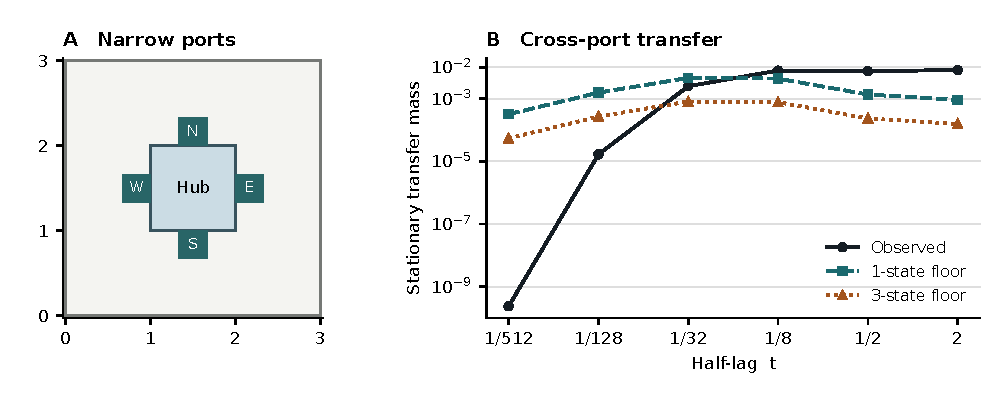
\includegraphics[width=.97\linewidth]{junction.pdf}
 \caption{Equilibrium diffusion with separated ports. The four dark patches in A are the measured ports. Panel B uses \(n=18\), \(D_x=D_y=1\), and \(w=1/3\). Observed mass below a floor excludes the corresponding hub budget. At half-lag \(1/32\) the data still exclude one state; at \(1/8\) the displayed floors both fall below the observation.}
 \label{fig:diffusion}
\end{figure}

For separated ports, the lower bound on the state count reached four in 19 of 42 configurations, three in two, two in three, and one in 18. For full-width ports it remained one in all 42. The trend with half-lag is visible in Figure~\ref{fig:diffusion}. At \(n=18,t=1/128\) in the isotropic separated case the observed mass was \(1.674\cdot10^{-5}\), compared with \(2.682\cdot10^{-4}\) required by any three-state hub and \(2.768\cdot10^{-3}\) predicted by repeating the one-step six-label kernel. In the full-width case at the same resolution and lag, the global prediction \(0.02811\) also exceeded the observed \(0.01827\), but the local one-state floor was only \(0.01145\). This discrepancy cannot be assigned to the hub by the all-pair test.

Enforcing the occupancy constraints increased the certified count in one of 84 configurations. At \(n=36,D_y=1/4,w=1/3,t=1/32\) the observed mass \(2.478\cdot10^{-4}\) lay between the relaxed and exact three-state floors, \(2.387\cdot10^{-4}\) and \(2.538\cdot10^{-4}\). At \(n=18\) in that same geometry the exact floor lay just below the observation. Thus the stronger four-state conclusion at this lag is sensitive to spatial resolution.


\section{Inference from independent endpoint counts}
Suppose the hub mass and port masses are known, for example from the cell volumes. In one ensemble, start \(N\) independent paths in the equilibrium distribution conditional on \(B\), and record their labels at \(t\). Each port count has marginal law \(\mathrm{Bin}(N,a_i/M)\). In a second ensemble, start \(N\) independent paths in the union of ports, again conditionally at equilibrium. Count a hit if the endpoint at \(2t\) lies in a port different from its starting port. For unit pair weights the hit probability is \(2Y/\pi(\cup_i A_i)\). This design directly estimates the small cross-port signal with one binomial count.

Form lower limits \(L_i\) on the masses \(a_i\) and an upper limit \(U\) on \(Y\), allocating error \(\alpha/(d+1)\) to each limit. We invert the one-sided Bernoulli Chernoff bound: on the relevant side of empirical fraction \(q\) use \(p\) satisfying
\[
 N\left[q\log(q/p)+(1-q)\log((1-q)/(1-p))\right]
 =\log((d+1)/\alpha)
\]
with the natural endpoints for all-zero or all-one counts. On the joint coverage event, monotonicity implies that \(U<\E_k(L,M;W)\) rules out \(k\) states. A union bound controls the probability of any false exclusion by \(\alpha\), simultaneously over all tested \(k\) at a specified lag. Counts within the hub multinomial need not be independent for this argument. Scanning lags or pair weights on noisy data would require simultaneous limits for those additional choices.

\begin{table}[htbp]
\centering
\caption{Number of repeats certifying each lower bound, with two ensembles of \(N\) independent endpoints per repeat. Each row contains 200 repeats. A count of one is the trivial lower bound.}
\label{tab:counts}
\begin{tabular}{lr rrrr}
\toprule
&&\multicolumn{4}{c}{Certified lower bound}\\
\cmidrule(l){3-6}
Data source & \(N\) & 1 & 2 & 3 & 4\\
\midrule
Diffusion & 1,000   & 200 & 0   & 0   & 0\\
           & 10,000  & 0   & 0   & 114 & 86\\
           & 100,000 & 0   & 0   & 0   & 200\\
\addlinespace
Three-state hub & 1,000   & 200 & 0   & 0   & 0\\
                & 10,000  & 1   & 167 & 32  & 0\\
                & 100,000 & 0   & 0   & 200 & 0\\
\bottomrule
\end{tabular}
\end{table}

Table~\ref{tab:counts} uses the fixed isotropic \(n=18,w=1/3,t=1/128\) design and \(\alpha=0.05\). We draw endpoint counts directly from the multinomial and binomial laws above. The three-state control takes the same \(a_i\) as the diffusion and attains \(\E_3\) by Theorem~\ref{thm:finite}, placing it on the exclusion boundary. The diffusion's population lower bound of four was recovered in 86 of 200 repeats at 10,000 trials per ensemble and in all 200 at 100,000. None of the 600 control repeats falsely excluded three. The probability guarantee follows from the joint limits; these simulated counts describe power at the stated design points.


\section{Interpretation and scope}
A sharp scalar minimum can answer a model-design question even when the full hidden dynamics are unidentifiable. In a reversible network surrogate, violating the two-lag inequality calls for extra states inside the chosen cell or a change in the model assumptions. Nonnegative conductances, exact flux at one lag and mass conservation elsewhere cannot remove that violation. The formulas also permit a design calculation before acquiring full trajectories: the balanced expression specifies the cross-port resolution needed to exclude a proposed budget.

The observed lower bound is capped by the number of ports, even for a continuum junction. Equality of the monitored statistic leaves other transition masses and higher lags unconstrained. Equation~\eqref{eq:finite} is exact for stationary reversible discrete-time kernels with deterministic aggregate labels. A continuous-time embedding, imposed connectivity, fixed external dynamics or a specified internal geometry can raise the minimum. For selected nonmetric costs the unconstrained-mass expression remains a valid finite-lag lower bound, while a fractional allocation can outperform every pure partition under finite occupancy. Enumerating partitions is practical for small neighborhoods and grows combinatorially with the number of ports.

The numerical study uses an analytically specified diffusion and independent ensemble counts. Using one correlated experimental trajectory would require a dependence model or another source of valid joint confidence limits. Non-equilibrium preparations and directional transport can change the midpoint identity. These distinctions delimit the model classes an experimental exclusion can address.

\paragraph{Data and code availability.}
The protocol, Python implementation, numerical tables and replication commands are available in the \href{https://github.com/fightforbelief/p2-coarse-junctions}{project repository}. All benchmark inputs are specified analytically.
\paragraph{Funding and interests.}
The authors received no specific funding for this work and declare no competing interests.

\begin{thebibliography}{9}
\bibitem{fredkin} D.~R. Fredkin and J.~A. Rice, \href{https://nvlpubs.nist.gov/nistpubs/jres/090/jresv90n6p517_A1b.pdf}{Aggregated Markov processes and channel gating kinetics}, J. Res. Natl. Bur. Stand. 90 (1985), 517--520.
\bibitem{noe} F. No\'e, H. Wu, J.-H. Prinz and N. Plattner, \href{https://arxiv.org/abs/1309.3220}{Projected and hidden Markov models for calculating kinetics and metastable states of complex molecules}, J. Chem. Phys. 139 (2013), 184114.
\bibitem{vidyasagar} M. Vidyasagar, \href{https://personal.utdallas.edu/~mxv091000/Research/hmm-full.pdf}{The complete realization problem for hidden Markov models: a survey and some new results}, Math. Control Signals Systems 23 (2011), 1--65.
\bibitem{duan} Y. Duan, M. Wang, Z. Wen and Y. Yuan, \href{https://doi.org/10.1137/18M1220790}{Adaptive low-nonnegative-rank approximation for state aggregation of Markov chains}, SIAM J. Matrix Anal. Appl. 41 (2020), 244--278.
\bibitem{cicalese} F. Cicalese, E. Laber and L. Murtinho, \href{https://proceedings.mlr.press/v97/cicalese19a.html}{New results on information theoretic clustering}, Proc. Mach. Learn. Res. 97 (2019), 1242--1251.
\bibitem{keller} M. Keller, D. Lenz, F. M\"unch, M. Schmidt and A. Telcs, \href{https://doi.org/10.1112/blms/bdw054}{Note on short-time behavior of semigroups associated to self-adjoint operators}, Bull. Lond. Math. Soc. 48 (2016), 935--944.
\end{thebibliography}
\end{document}
